\section{Auswertung}
\label{sec:Auswertung}
\subsection{Beugung am Einzelspalt}
In diesem Kapitel wird mit den aufgenommenen Messwerten die Beugungsfigur zweier Einzelspalte graphisch dargestellt.
Außerdem wird die Spaltbreite $b$ experimentell bestimmt.
Beim ersten Versuchsaufbau wurde der Spalt-Dioden Abstand $L$ gewählt. Der Abstand, die Wellenlänge
des benutzten Lasers $\lambda$, sowie, der zum Anfang gemessene Dunkelstrom $I_\text{dunkel}$ betragen:
\begin{align*}
  L_1 &= 1,00\,\si{\meter} \\
  \lambda &= 635\,\si{\nano\meter} \\
  I_\text{dunkel} &= 0,32\,\si{\nano\ampere}.
\end{align*}
Der Dunkelstrom wird bei der Bestimmung der Spaltbreite und bei allen graphischen
Darstellung der Beugungsfiguren von der gemessenen Lichtintensität abgezogen. Es wird angenommen, dass dieser in der kompletten
Messreihe konstant ist.
Die Ausgleichsrechnung für den Einzelspalt wird mit Gleichung xyz berechnet. Der Winkel $\phi$ ist approximiert
das Verhältnis zwischen dem Abstand $x$ in der Bildebene des Intereferenzmusters und $L$ der Spalt-Dioden Länge, also:
\begin{align*}
\phi \approx \frac{x}{L}.
\end{align*}
Die Beugungsfigur, also die Messwerte und die Ausgleichsrechnung, befinden sich in Abbildung \ref{fig:einzel1}
und die Messpaare befinden sich in Tabelle \ref{tab:einzel1}.


\begin{figure}[H]
  \center
  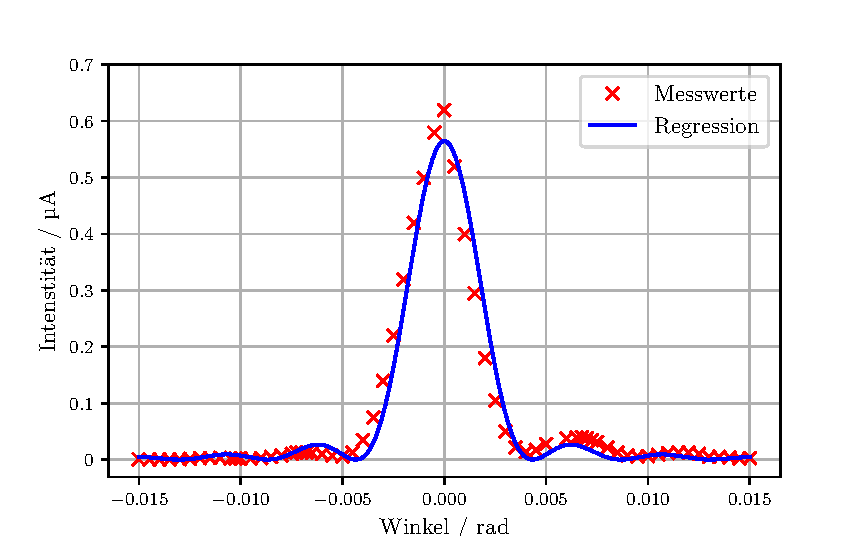
\includegraphics[scale = 0.75]{einzel1.pdf}
  \caption{Beugungsfigur am Einzelspalt mit Spaltbreite $b_\text{1,th} = 0,15\,\si{\milli\meter}$.}
  \label{fig:einzel1}
\end{figure}

%Tabelle 1
\begin{table}
\centering
\caption{Die für die Bestimmung der Spaltbreite $b_\text{1,exp}$ benötigten Messpaare.}
\label{tab:einzel1}
\begin{tabular}{c c c c}
\toprule
$x\:/\: \si{\milli\meter}$ & $I\:/\: \si{\micro\ampere}$ &
$x\:/\: \si{\milli\meter}$ & $I\:/\: \si{\micro\ampere}$ \\
\midrule
\num{-15  } & 0.00064  & 0.0     & 0.62  \\
\num{-14.5} & 0.00064  & 0.5     & 0.52  \\
\num{-14  } & 0.00075  & 1       & 0.4  \\
\num{-13.5} & 0.0008   & 1.5     & 0.295  \\
\num{-13  } & 0.0012   & 2       & 0.18  \\
\num{-12.5} & 0.0018   & 2.5     & 0.105  \\
\num{-12  } & 0.0026   & 3       & 0.05  \\
\num{-11.5} & 0.0032   & 3.5     & 0.0218  \\
\num{-11  } & 0.0033   & 4       & 0.014  \\
\num{-10.5} & 0.00295  & 4.5     & 0.018  \\
\num{-10.2} & 0.0027   & 5       & 0.028  \\
\num{-10  } & 0.0024   & 6       & 0.037  \\
\num{-9.5}  & 0.0022   & 6.5     & 0.04  \\
\num{-9   } & 0.0027   & 6.75    & 0.04  \\
\num{-8.5}  & 0.0052   & 7       & 0.038  \\
\num{-8   } & 0.00765  & 7.25    & 0.035  \\
\num{-7.5}  & 0.0105   & 7.5     & 0.031  \\
\num{-7.25} & 0.0125   & 8       & 0.022  \\
\num{-7   } & 0.013    & 8.5     & 0.0135  \\
\num{-6.75} & 0.013    & 9       & 0.0075  \\
\num{-6.5}  & 0.0125   & 9.5     & 0.0057  \\
\num{-6   } & 0.0105   & 10      & 0.0066  \\
\num{-5.5}  & 0.007    & 10.5    & 0.0092  \\
\num{-5   } & 0.006    & 11      & 0.012  \\
\num{-4.5}  & 0.013    & 11.5    & 0.013  \\
\num{-4   } & 0.035    & 12      & 0.0125  \\
\num{-3.5}  & 0.075    & 12.5    & 0.0105  \\	
\num{-3	  } & 0.14     & 13      & 0.0051  \\
\num{-2.5}  & 0.22     & 13.5    & 0.005  \\	
\num{-2	  } & 0.32     & 14      & 0.0035  \\
\num{-1.5}  & 0.42     & 14.5    & 0.0028  \\	
\num{-1	  } & 0.5      & 15      & 0.003  \\
\num{-0.5}  & 0.58     & 	& \\
\bottomrule
\end{tabular}
\end{table}

\noindent Mit der Ausgleichsrechnung ergibt sich die Spaltbreite
\begin{align*}
b_\text{1,exp} &= (\num{0.1462 +- 0.0035})\,\si{\milli\meter}.
\end{align*}

\noindent Beim zweiten Versuchsaufbau wurde derselbe Spalt-Dioden Abstand gewählt. Auch die Vorgehensweise
bei diesem etwas breiteren Einzelspalt ist die selbe wie zuvor. Die Ausgleichsrechnung wird erneut mit Gleichung xyz
durchgeführt. Die Beugungsfigur befindet sich in Abbildung \ref{fig:einzel2} und die Messpaare befinden sich in Tabelle \ref{tab:einzel2}.

\begin{figure}[H]
  \center
  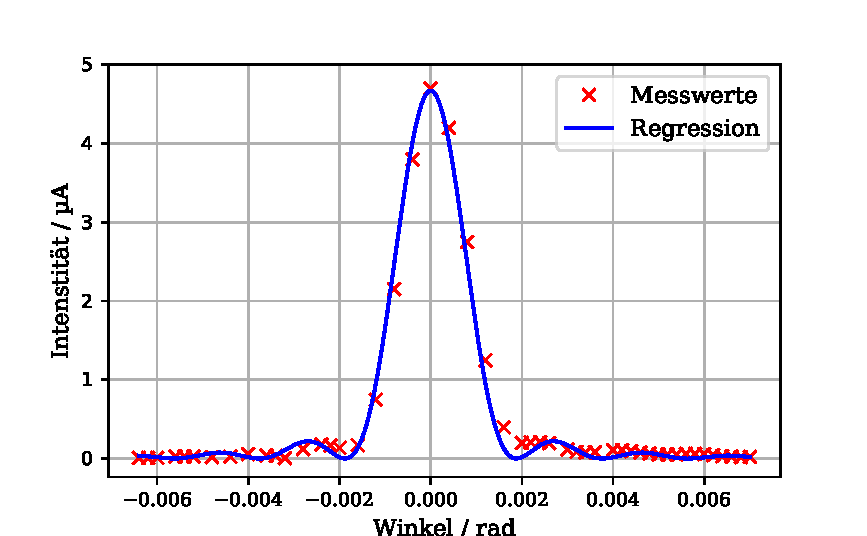
\includegraphics[scale = 0.75]{einzel2.pdf}
  \caption{Beugungsfigur am Einzelspalt mit Spaltbreite $b_\text{2,th} = 0,4\,\si{\milli\meter}$.}
  \label{fig:einzel2}
\end{figure}

%Tabelle 2
\begin{table}[H]
\centering
\caption{Die für die Bestimmung der Spaltbreite $b_\text{2,exp}$ benötigten Messpaare.}
\label{tab:einzel2}
\begin{tabular}{c c c c}
\toprule
$x\:/\: \si{\milli\meter}$ & $I\:/\: \si{\micro\ampere}$ &
$x\:/\: \si{\milli\meter}$ & $I\:/\: \si{\micro\ampere}$ \\
\midrule
\num{-6.4} & 0.011 & \num{2.0}  & 0.2 \\
\num{-6.2} & 0.01 & \num{2.2}   & 0.205 \\
\num{-6.0} & 0.012 & \num{2.4}  & 0.21 \\
\num{-5.6} & 0.0225 & \num{2.6} & 0.195 \\
\num{-5.4} & 0.025 & \num{3.0}  & 0.12 \\
\num{-5.2} & 0.024 & \num{3.2}  & 0.084 \\
\num{-4.8} & 0.0175 & \num{3.4} & 0.074 \\
\num{-4.4} & 0.026 & \num{3.6}  & 0.081 \\
\num{-4.0} & 0.058 & \num{4.0}  & 0.105 \\
\num{-3.6} & 0.042 & \num{4.2}  & 0.105 \\
\num{-3.4} & 0.035 & \num{4.4}  & 0.095 \\
\num{-3.2} & 0.005 & \num{4.6}  & 0.075 \\
\num{-2.8} & 0.12 & \num{4.8}   & 0.06 \\
\num{-2.4} & 0.18 & \num{5.0}   & 0.05 \\
\num{-2.2} & 0.165 & \num{5.2}  & 0.0495 \\
\num{-2.0} & 0.135 & \num{5.4}  & 0.052 \\
\num{-1.6} & 0.17 & \num{5.6}   & 0.06 \\
\num{-1.2} & 0.75 & \num{5.8}   & 0.062 \\
\num{-0.8} & 2.15 & \num{6.0}   & 0.056 \\
\num{-0.4} & 3.8 & \num{6.2}    & 0.044 \\
\num{0.0}  & 4.7  & \num{6.4}   & 0.032 \\
\num{0.4}  & 4.2  & \num{6.6}   & 0.023 \\
\num{0.8}  & 2.75  & \num{6.8}  & 0.02 \\
\num{1.2}  & 1.25  & \num{7.0}  & 0.022 \\
\num{1.6}  & 0.4  & & \\
\bottomrule
\end{tabular}
\end{table}

\noindent Mit der Ausgleichsrechnung ergibt sich die Spaltbreite
\begin{align*}
b_\text{2,exp} &= (\num{0.338 +- 0.005}) \,\si{\milli\meter}.
\end{align*}

\subsection{Beugung am Doppelspalt und Vergleich}
Mithilfe der aufgenommenen Messwerte, welche in Tabelle \ref{tab:doppel} dargestellt sind,
wird das Beugungsmuster eines Doppelspalts erstellt. Eine Ausgleichsrechnung nach Gleichung (5)
wird durchgeführt und beide werden in Abbildung \ref{fig:doppel} dargestellt.

\begin{figure}[H]
  \center
  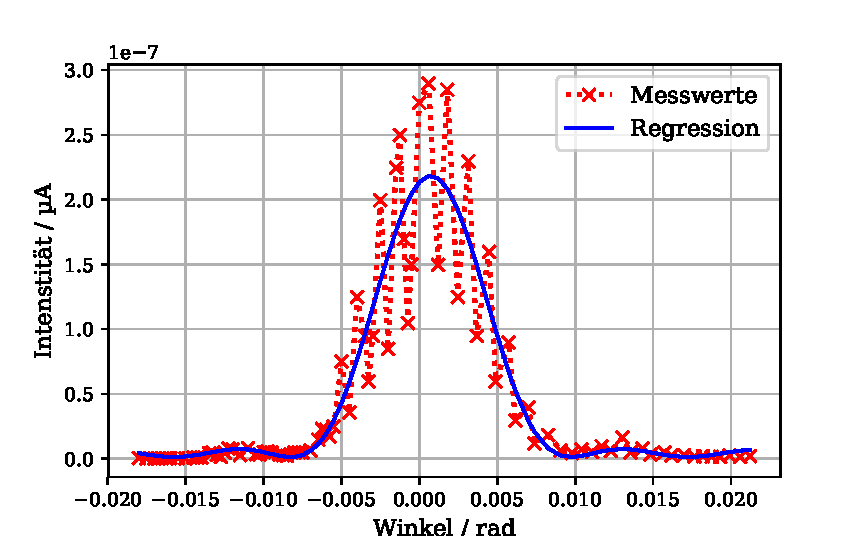
\includegraphics[scale = 0.75]{doppel.pdf}
  \caption{Beugungsfigur am Doppelspalt mit Spaltbreite $b_3 = 0,1\,\si{\milli\meter}$ und Abstand $s = 0,4\,\si{\milli\meter}$.}
  \label{fig:doppel}
\end{figure}

%Tabelle 3
\begin{table}
\centering
\caption{Messdaten des Beugungsmusters des Doppelspalts.}
\label{tab:doppel}
\begin{tabular}{c c c c c c}
\toprule
$x\:/\: \si{\milli\meter}$ & $I\:/\: \si{\micro\ampere}$ &
$x\:/\: \si{\milli\meter}$ & $I\:/\: \si{\micro\ampere}$ &
$x\:/\: \si{\milli\meter}$ & $I\:/\: \si{\micro\ampere}$ \\
\midrule
-1.8   & 0.00064  & -0.775 & 0.0053   & 0.573   & 0.09\\
-1.75  & 0.0006   & -0.75  & 0.0051   & 0.616   & 0.03\\
-1.7   & 0.00064  & -0.7   & 0.0064   & 0.700   & 0.04\\
-1.675 & 0.00066  & -0.65  & 0.015    & 0.740   & 0.012 \\
-1.65  & 0.00063  & -0.625 & 0.0235   & 0.827   & 0.0185 \\
-1.625 & 0.0006   & -0.6   & 0.0225   & 0.907   & 0.0065 \\
-1.6   & 0.00062  & -0.575 & 0.0175   & 0.977   & 0.0046 \\
-1.55  & 0.00074  & -0.55  & 0.025    & 1.040   & 0.0072 \\
-1.5   & 0.000515 & -0.5   & 0.075    & 1.109   & 0.0055 \\
-1.45  & 0.001    & -0.45  & 0.036    & 1.169   & 0.01 \\
-1.425 & 0.00115  & -0.4   & 0.125    & 1.229   & 0.0063 \\
-1.4   & 0.0012   & -0.35  & 0.095    & 1.304   & 0.0165 \\
-1.35  & 0.0043   & -0.325 & 0.06     & 1.355   & 0.005 \\
-1.325 & 0.005    & -0.3   & 0.095    & 1.430   & 0.008 \\
-1.3   & 0.0031   & -0.25  & 0.2      & 1.483   & 0.0035 \\
-1.275 & 0.0016   & -0.2   & 0.085    & 1.573   & 0.005 \\
-1.25  & 0.0047   & -0.15  & 0.225    & 1.618   & 0.0025 \\
-1.225 & 0.0078   & -0.125 & 0.25     & 1.698   & 0.0028 \\
-1.2   & 0.0072   & -0.1   & 0.17     & 1.763   & 0.002 \\
-1.15  & 0.003    & -0.075 & 0.105    & 1.820   & 0.00225 \\
-1.1   & 0.0084   & -0.05  & 0.15     & 1.877   & 0.00185 \\
-1.05  & 0.0038   & 0      & 0.275    & 1.930   & 0.0018 \\
-1.025 & 0.0035   & 0.060  & 0.29     & 1.990   & 0.00245 \\
-1     & 0.0054   & 0.120  & 0.15     & 2.060   & 0.00155 \\
-0.975 & 0.006    & 0.180  & 0.285    & 2.120   & 0.0022\\
-0.95  & 0.005    & 0.246  & 0.125    & &\\
-0.9   & 0.0035   & 0.314  & 0.23     & &\\
-0.875 & 0.0028   & 0.367  & 0.095    & &\\
-0.85  & 0.0026   & 0.447  & 0.16     & &\\
-0.8   & 0.0052   & 0.490  & 0.06     & &\\
\bottomrule
\end{tabular}
\end{table}

Zuletzt wird die Beugungsfigur des ersten Einzelspalts mit einer skalierten Beugungsfigur des Doppelspalts
in Abbildung \ref{fig:vergleich} dargestellt.

\begin{figure}[H]
  \center
  \includegraphics[scale = 0.75]{Vergleich.pdf}
  \caption{Skalierte Beugungsfigur des Doppelspalts und des ersten Einzelspalts.}
  \label{fig:vergleich}
\end{figure}